%!TEX root = ../larxxia.tex
\section{The cross product}
\label{sec:cp}
\secttoc

\index{cross product|(}


In the three dimensions of the world we live in, 
\begin{aside}
This section is optional, 
but is vital in many topics of science and engineering.
\end{aside}
as well as the dot product there is another way to multiply vectors, called the cross product.
For more than three dimensions, qualitatively different techniques are developed in subsequent chapters.


\subsubsection{Area of a parallelogram}


\begin{wrapfigure}{r}{0pt} 
\begin{tikzpicture} 
\def\a{2} \def\b{0.5} \def\ab{2.5}
\def\c{1} \def\d{1.5} \def\cd{2.5}
\begin{axis}[axis equal image, axis lines=middle
    ,xtick={\a,\b,\ab},xticklabels={$v_1$,$w_1$,$v_1+w_1$}
    ,ytick={\c,\d,\cd},yticklabels={$v_2$,$w_2$,$v_2+w_2$}
    ,xmax=3,ymax=2.8,small
    ]
    \addplot[quiver={u=\a,v=\c},blue,-stealth] 
    coordinates {(0,0)(\b,\d)};
    \node[left] at (axis cs:\a,\c) {\small$(v_1,v_2)$};
    \addplot[quiver={u=\b,v=\d},blue,-stealth] 
    coordinates {(0,0)(\a,\c)};
    \node[right] at (axis cs:\b,\d) {\small$(w_1,w_2)$};
    \node[above] at (axis cs:\ab,\cd) {\small$(v_1+w_1,v_2+w_2) \hspace*{3.5em}$};
    \addplot[brown] coordinates {(\ab,0)(\ab,\cd)(0,\cd)};
    \addplot[brown] coordinates {(\ab,0)(\ab,\c)(\a,\c)(\a,0)};
    \addplot[brown] coordinates {(0,\cd)(\b,\cd)(\b,\d)(0,\d)};
\end{axis}
\end{tikzpicture}
\end{wrapfigure}
Consider the parallelogram drawn in blue.
It has sides given by vectors \(\vv=(v_1,v_2)\) and \(\wv=(w_1,w_2)\) as shown.
Let's determine the area of the parallelogram by that of the containing rectangle less the two small rectangles and the four small triangles.
The two small rectangles have the same area, namely~\(w_1v_2\).
The two small triangles on the left and the right also have the same area, namely~\(\frac12w_1w_2\).
The two small triangles on the top and the bottom similarly have the same area, namely~\(\frac12v_1v_2\).
Thus, the parallelogram has 
\begin{eqnarray*}
\text{area}&=&(v_1+w_1)(v_2+w_2)-2w_1v_2-2\cdot\frac12w_1w_2-2\cdot\frac12v_1v_2
\nonumber
\\&=&v_1v_2+v_1w_2+w_1v_2+w_1w_2-2w_1v_2-w_1w_2-v_1v_2
\nonumber
\\&=&v_1w_2-v_2w_1\,. %\label{eq:cppara}
\end{eqnarray*}
In application, sometimes this right-hand side expression is negative because vectors~\vv\ and~\wv\ are the `wrong way' around.
Thus in general the \idx{parallelogram area}\({}=|v_1w_2-v_2w_1|\).



\begin{example} \label{eg:}
What is the area of the parallelogram (illustrated in the margin) whose edges are formed by the vectors~\((3,2)\) and~\((-1,4)\)?
\marginpar{\begin{tikzpicture} 
\def\a{3} \def\b{-1} 
\def\c{2} \def\d{4} 
\begin{axis}[footnotesize,font=\footnotesize,axis equal image, axis lines=middle
    ,xmin=-2.9,xmax=3.5,ymax=6.5
    ]
    \addplot[quiver={u=\a,v=\c},blue,-stealth] 
    coordinates {(0,0)(\b,\d)};
    \node[left] at (axis cs:\a,\c) {$(\a,\c)$};
    \addplot[quiver={u=\b,v=\d},blue,-stealth] 
    coordinates {(0,0)(\a,\c)};
    \node[above] at (axis cs:\b,\d) {$(\b,\d)\qquad$};
\end{axis}
\end{tikzpicture}}
\begin{solution} 
The parallelogram area\({}=|3\cdot4-2\cdot(-1)|=|12+2|=14\)\,.  
The illustration indicates that this area must be about right as with imagination one could cut the area and move it about to form a rectangle roughly~\(3\) by~\(5\), and hence the area should be roughly~\(15\).
\end{solution}
\end{example}



\begin{activity} \label{ex:} 
What is the area of the parallelogram (illustrated in the margin) whose edges are formed by the vectors~\((5,3)\) and~\((2,-2)\)?
\marginpar{\begin{tikzpicture} 
\def\a{5} \def\b{2} \def\ab{7}
\def\c{3} \def\d{-2} \def\cd{1}
\begin{axis}[footnotesize,font=\footnotesize
    ,axis equal image, axis lines=middle
    ,ymin=-2.5,ymax=3.5,xmax=7.5
    ]
    \addplot[quiver={u=\a,v=\c},blue,-stealth] 
    coordinates {(0,0)(\b,\d)};
    \node[left] at (axis cs:\a,\c) {$(\a,\c)$};
    \addplot[quiver={u=\b,v=\d},blue,-stealth] 
    coordinates {(0,0)(\a,\c)};
    \node[right] at (axis cs:\b,\d) {$(\b,\d)$};
\end{axis}
\end{tikzpicture}}
\partswidth=7em
\begin{parts}
\item \(-16\)
\item \(-4\)
\item \(4\)
\item \(11\)
\item \(16\)
\item \(19\)
\end{parts}
\end{activity}


Interestingly, we meet this expression for area, \(v_1w_2-v_2w_1\), in another context: that of equations for a plane and its normal vector.





\subsubsection{Normal vector to a plane}
Recall section~\ref{sec:nvep} introduced that we describe planes either via an equation such as \(x-y+3z=6\) or via a parametric description such as \(\xv=(1,1,2)+(1,1,0)s+(0,3,1)t\)\,.
These determine the same plane, just different algebraic descriptions.
One converts between these two descriptions using the cross product.




\begin{example} \label{eg:nviax}
Derive that the plane described parametrically by \(\xv=(1,1,2)+(1,1,0)s+(0,3,1)t\) has normal equation \(x-y+3z=6\)\,.
\begin{solution} 
They key to deriving the normal equation is to find that a \idx{normal vector} to the plane is~\((1,-1,3)\).
This normal vector comes from the two vectors that multiply the parameters in the parametric form, \((1,1,0)\) and~\((0,3,1)\).
(Those who have seen \(3\times3\) determinants will recognise the following has the same pattern---see Chapter~\ref{ch:ddm}.)
Write the vectors as two consecutive columns, following a first column of the \emph{symbols} of the standard unit vectors~\iv, \jv\ and~\kv, in
\setlength{\unitlength}{1.2ex}
\def\abc#1{\begin{vmatrix}\begin{picture}(5.3,6)
%\put(0,0){\framebox(5,5){}}
\put(0,4){$\iv$}\put(2,4){$1$}\put(4,4){$0$}
\put(0,2){$\jv$}\put(2,2){$1$}\put(4,2){$3$}
\put(0,0){$\kv$}\put(2,0){$0$}\put(4,0){$1$}
\ifnum1=#1\put(0.5,-0.5){\line(0,1)6}\put(-0.5,4.5){\line(1,0)6}\fi
\ifnum2=#1\put(0.5,-0.5){\line(0,1)6}\put(-0.5,2.5){\line(1,0)6}\fi
\ifnum3=#1\put(0.5,-0.5){\line(0,1)6}\put(-0.5,0.5){\line(1,0)6}\fi
\end{picture}\end{vmatrix}}
\def\ab#1#2#3#4{\begin{vmatrix}\begin{picture}(3,4)
\put(0,2){$#1$}\put(2,2){$#2$}
\put(0,0){$#3$}\put(2,0){$#4$}
\color{red}\put(-0.5,-0.5){\line(1,1)4}
\color{blue}\put(-0.5,3.5){\line(1,-1)4}
\end{picture}\end{vmatrix}}
\begin{eqnarray*}
\nv&=& \abc0 
\\&&\parbox{20em}{(cross out 1st column and each row, multiplying each by common entry, with alternating sign)}
\\&=&\iv\abc1-\jv\abc2+\kv\abc3
\\&=&\iv\begin{vmatrix} 1&3\\0&1 \end{vmatrix}
-\jv\begin{vmatrix} 1&0\\0&1 \end{vmatrix}
+\kv\begin{vmatrix} 1&0\\1&3 \end{vmatrix}
\\&&\parbox{20em}{(draw diagonals, then subtract product of red diagonal from product of the blue)}
\\&=&\iv\ab1301
-\jv\ab1001
+\kv\ab1013
\\&=&\iv(1\cdot1-0\cdot3)
-\jv(1\cdot1-0\cdot0)
+\kv(1\cdot3-1\cdot0)
\\&=&\iv-\jv+3\kv\,.
\end{eqnarray*}
Using this normal vector, the equation of the plane must be of the form \(x-y+3z={}\)constant.
Since the plane goes through point~\((1,1,2)\), the constant\({}=1-1+3\cdot2=6\); that is, the plane is \(x-y+3z=6\) (as given).
\end{solution}
\end{example}




\begin{activity} \label{ex:} 
Use the procedure of Example~\ref{eg:nviax} to derive a \idx{normal vector} to the plane described in parametric form as \(\xv=(4,-1,-2)+(1,-2,1)s+(2,-3,-2)t\).  
Which of the following is your computed normal vector?
%pqr=0+round(randn(3)*2),n=cross(pqr(2,:),pqr(3,:))
\begin{parts}
\item \((5,6,7)\)
\item \((7,4,1)\)
\item \((-4,4,-10)\)
\item \((2,-2,5)\)
\item \((-7,-4,-1)\)
\item \((-4,-3,3)\)
\end{parts}
\end{activity}




\subsubsection{Definition of a cross product}

\paragraph{General formula}
The procedure used in Example~\ref{eg:nviax} to derive a \idx{normal vector} leads to an algebraic formula.  
Let's apply the same procedure to two general vectors \(\vv=(v_1,v_2,v_3)\) and \(\wv=(w_1,w_2,w_3)\).
The procedure computes
{%%%%%%%%%%%%%%%%%%
\setlength{\unitlength}{1.3ex}
\def\abc#1{\begin{vmatrix}\begin{picture}(6.3,6)
%\put(0,0){\framebox(5,5){}}
\put(0,4){$\iv$}\put(2,4){$v_1$}\put(4,4){$w_1$}
\put(0,2){$\jv$}\put(2,2){$v_2$}\put(4,2){$w_2$}
\put(0,0){$\kv$}\put(2,0){$v_3$}\put(4,0){$w_3$}
\ifnum1=#1\put(0.5,-0.5){\line(0,1)6}\put(-0.5,4.5){\line(1,0)6}\fi
\ifnum2=#1\put(0.5,-0.5){\line(0,1)6}\put(-0.5,2.5){\line(1,0)6}\fi
\ifnum3=#1\put(0.5,-0.5){\line(0,1)6}\put(-0.5,0.5){\line(1,0)6}\fi
\end{picture}\end{vmatrix}}
\def\ab#1#2{\begin{vmatrix}\begin{picture}(4,4)
\put(0,2){$v_#1$}\put(2,2){$w_#1$}
\put(0,0){$v_#2$}\put(2,0){$w_#2$}
\color{red}\put(-0.5,-0.5){\line(1,1)4}
\color{blue}\put(-0.5,3.5){\line(1,-1)4}
\end{picture}\end{vmatrix}}
\begin{eqnarray*}
\nv&=& \abc0 
\\&&\parbox{20em}{(cross out 1st column and each row, multiplying each by common entry, with alternating sign)}
\\&=&\iv\abc1-\jv\abc2+\kv\abc3
\\&=&\iv\begin{vmatrix} v_2&w_2\\v_3&w_3 \end{vmatrix}
-\jv\begin{vmatrix} v_1&w_1\\v_3&w_3 \end{vmatrix}
+\kv\begin{vmatrix} v_1&w_1\\v_2&w_2 \end{vmatrix}
\\&&\parbox{20em}{(draw diagonals, then subtract product of red diagonal from product of the blue)}
\\&=&\iv\ab23
-\jv\ab13
+\kv\ab12
\\&=&\iv(v_2w_3-v_3w_2)
-\jv(v_1w_3-v_3w_1)
+\kv(v_1w_2-v_2w_1).
\end{eqnarray*}
}%%%%%%%%%%%%%%%%%%%%
We use this formula to define the cross product algebraically, and then see what it means geometrically.

\begin{definition} \label{def:cp}
Let \(\vv=(v_1,v_2,v_3)\) and \(\wv=(w_1,w_2,w_3)\) be any two vectors in~\(\RR^3\).
The \bfidx{cross product}  (or \bfidx{vector product}) \(\vv\times\wv\) is defined algebraically as
\begin{equation*}
\vv\times\wv:=\iv(v_2w_3-v_3w_2)
+\jv(v_3w_1-v_1w_3)
+\kv(v_1w_2-v_2w_1).
\end{equation*}
\end{definition}



\begin{example} \label{eg:cpijk}
Among the \idx{standard unit vector}s, derive that 
\begin{parts}
\item \(\iv\times\jv=\kv\)\,, \item \(\jv\times\iv=-\kv\)\,,
\item \(\jv\times\kv=\iv\)\,, \item \(\kv\times\jv=-\iv\)\,,
\item \(\kv\times\iv=\jv\)\,, \item \(\iv\times\kv=-\jv\)\,,
\item \(\iv\times\iv=\jv\times\jv=\kv\times\kv=\ov\)\,.
\end{parts}
\begin{solution} Using Definition~\ref{def:cp}:
\begin{eqnarray*}
\iv\times\jv&=&(1,0,0)\times(0,1,0)
\\&=&\iv(0\cdot0-0\cdot1)
+\jv(0\cdot0-1\cdot0)
+\kv(1\cdot1-0\cdot0)
\\&=&\kv\,;
\\\jv\times\iv&=&(0,1,0)\times(1,0,0)
\\&=&\iv(1\cdot0-0\cdot0)
+\jv(0\cdot1-0\cdot0)
+\kv(1\cdot1-1\cdot1)
\\&=&-\kv\,;
\\\iv\times\iv&=&(1,0,0)\times(1,0,0)
\\&=&\iv(0\cdot0-0\cdot0)
+\jv(0\cdot1-1\cdot0)
+\kv(1\cdot0-0\cdot1)
\\&=&\ov\,.
\end{eqnarray*}
Exercise~\ref{ex:cpijk} asks you to correspondingly establish the other six identities.
\end{solution}
These example cross products most clearly demonstrate the orthogonality of a cross product to its two argument vectors (Theorem~\ref{thm:cpga}) and that the direction is in the right-hand sense (Theorem~\ref{thm:cpgb}).
\end{example}




\begin{activity} 
Use the Definition~\ref{def:cp} to find the cross product of \((-4,1,-1)\) and \((-2,2,1)\) is which one of the following:
\begin{parts}
\item \((-3,-6,6)\),
\item \((3,-6,-6)\),
\item \((-3,-6,6)\),
\item \((3,6,-6)\).
\end{parts}
\end{activity}




\subsubsection{Geometry of a cross product}


\begin{example}[\idx{parallelogram area}] \label{eg:cppara}
Let's revisit the introduction to this section.
Consider the parallelogram in the \(x_1x_2\)-plane with edges formed by the \(\RR^3\)~vectors \(\vv=(v_1,v_2,0)\) and \(\wv=(w_1,w_2,0)\).
At the start of this Section~\ref{sec:cp} we derived that the parallelogram formed by these vectors has area\({}=|v_1w_2-v_2w_1|\).
Compare this area with the cross product
\begin{eqnarray*}
\vv\times\wv&=&\iv(v_2\cdot0-0\cdot w_2)
+\jv(0\cdot w_1-v_1\cdot0)
+\kv(v_1w_2-v_2w_1)
\\&=&\iv0+\jv0+\kv(v_1w_2-v_2w_1)
\\&=&\kv(v_1w_2-v_2w_1).
\end{eqnarray*}
Consequently, the length of this cross product equals the area of the parallelogram formed by~\vv\ and~\wv\ (Theorem~\ref{thm:cpgd}).
(Also the direction of the cross product,~\(\pm\kv\), is orthogonal to the \(x_1x_2\)-plane containing the two vectors---Theorem~\ref{thm:cpga}).
\end{example}



\begin{activity}
Using property~\ref{thm:cpgb} of the next theorem, in which direction is the cross product \(\vv\times\wv\) for the two vectors illustrated in stereo below?
\begin{center}
\qview{30}{35}{\begin{tikzpicture} 
\begin{axis}[footnotesize,font=\footnotesize,axis equal,view={\q}{30}
    ,xlabel={$x_1$},ylabel={$x_2$},zlabel={$x_3$},label shift={-1.5ex}
    ]
    \threev[above]20{0.5}{\vec v};
    \threev[above]102{\vec w};
\end{axis}
\end{tikzpicture}}
\end{center}
\partswidth=3em
\begin{parts}
\item \(+\iv\) \item \(+\jv\) \item \(+\kv\) 
\item \(-\iv\) \item \(-\jv\) \item \(-\kv\) 
\end{parts}
\end{activity}




\begin{theorem}[cross product geometry] \label{thm:cpg}
Let \vv\ and~\wv\ be any two vectors in~\(\RR^3\):
\begin{enumerate}
\item\label{thm:cpga} the vector~\(\vv\times\wv\) is \idx{orthogonal} to both~\vv\ and~\wv;

\item\label{thm:cpgb} the \index{cross product direction}direction of~\(\vv\times\wv\) is in the right-hand sense%
%\marginpar{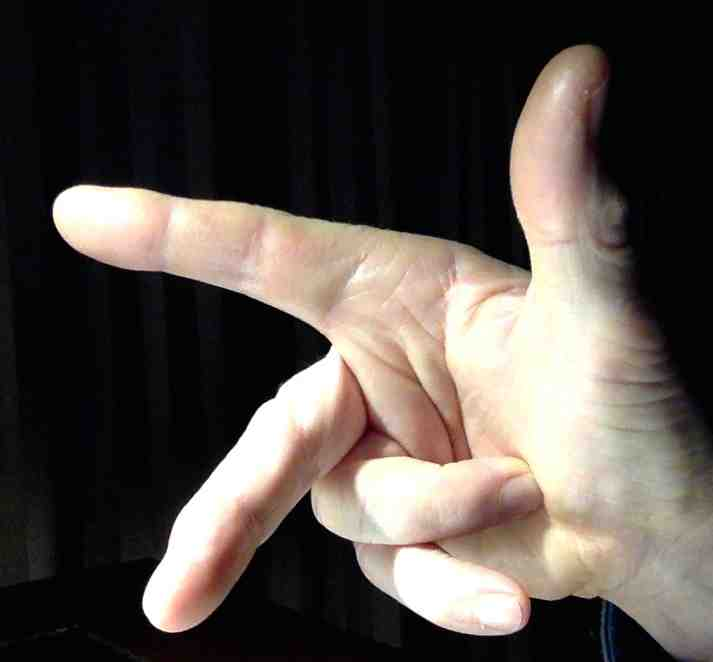
\includegraphics[width=7em]{Vectors/right-hand-rule}}
\marginpar{\begin{tikzpicture}
  \begin{axis}[small,thick, axis lines=none,ymax=1.3,ymin=-0.3,xmin=-0.3,xmax=1.3]
    \addplot graphics [xmin=0,xmax=1,ymin=0,ymax=1]
      {Vectors/right-hand-rule.jpg};
    \addplot[blue,quiver={u=-0.05,v=0.5,scale arrows=1.07},-stealth] coordinates {(0.55,0.55)};
    \node[above] at (axis cs:0.5,1.05) {$\vv$};
    \addplot[blue,quiver={u=-0.6,v=0.2,scale arrows=1.07},-stealth] coordinates {(0.55,0.55)};
    \node[left] at (axis cs:-0.05,0.77) {$\wv$};
    \addplot[blue,quiver={u=-0.4,v=-0.6,scale arrows=1.07},-stealth] coordinates {(0.55,0.55)};
    \node[below] at (axis cs:0.15,-0.05) {$\vv\times\wv$};
  \end{axis}
\end{tikzpicture}}
in that if \vv~is in the direction of your thumb, and \wv~is in the direction of your straight index finger, then \(\vv\times\wv\) is in the direction of your bent second\slash longest finger---all on your right-hand as illustrated in the margin; 

\item\label{thm:cpgc} \(|\vv\times\wv|=|\vv|\,|\wv|\sin\theta\) where \(\theta\)~is the \idx{angle} between vectors~\vv\ and~\wv\ (\(0\leq\theta\leq\pi\), equivalently \(0^\circ\leq\theta\leq180^\circ\)); and

\item\label{thm:cpgd} the \idx{length}~\(|\vv\times\wv|\) is the \idx{area} of the parallelogram\index{parallelogram area} with edges~\vv\ and~\wv.
\end{enumerate}
\end{theorem}


\begin{proof} 
Let \(\vv=(v_1,v_2,v_3)\) and \(\wv=(w_1,w_2,w_3)\).
\begin{enumerate}
\item[\ref{thm:cpga}] Recall that two vectors are orthogonal if their dot product is zero (Definition~\ref{def:orthovec}).
To determine orthogonality between~\vv\ and the cross product \(\vv\times\wv\), consider
\begin{eqnarray*}
\vv\cdot(\vv\times\wv)
&=&(v_1\iv+v_2\jv+v_3\kv)
\cdot\big[\iv(v_2w_3-v_3w_2)
\\&&{}
+\jv(v_3w_1-v_1w_3)
+\kv(v_1w_2-v_2w_1)\big]
\\&=&v_1(v_2w_3-v_3w_2)
+v_2(v_3w_1-v_1w_3)
\\&&{}
+v_3(v_1w_2-v_2w_1)
\\&=&v_1v_2w_3-v_1v_3w_2
+v_2v_3w_1
\\&&{}
-v_1v_2w_3
+v_1v_3w_2-v_2v_3w_1
\quad{}=0
\end{eqnarray*}
as each term in the penultimate line cancels with the term underneath in the last line.
Since the dot product is zero, the cross product \(\vv\times\wv\) is orthogonal to vector~\vv.

Similarly, \(\vv\times\wv\) is orthogonal to~\wv\  (Exercise~\ref{ex:cpga}).

\item[\ref{thm:cpgb}] This right-handed property follows from the convention that the standard unit vectors~\iv, \jv\ and~\kv\ are right-handed: that if \iv~is in the direction of your thumb, and \jv~is in the direction of your straight index finger, then \kv~is in the direction of your bent second\slash longest finger---all on your right-hand.

We prove only for the case of vectors in the \(x_1x_2\)-plane, in which case \(\vv=(v_1,v_2,0)\) and \(\wv=(w_1,w_2,0)\), and when both \(v_1,w_1>0\)\,.
One example is in stereo below.
\begin{center}
\qview{30}{35}{\begin{tikzpicture} 
\def\a{1.5} \def\b{0.5} 
\def\c{1} \def\d{2} 
\begin{axis}[footnotesize,font=\footnotesize,axis equal,view={\q}{30}
    ,xmin=-0.4,xmax=2.4,ymin=-0.4,ymax=2.4,xtick={0,1,2},ztick={0,1}
    ,xlabel={$x_1$},ylabel={$x_2$},zlabel={$x_3$},label shift={-1.5ex}
    ]
    \addplot3[quiver={u=\a,v=\c,w=0},blue,-stealth,thick] 
    coordinates {(0,0,0)};
    \node[right] at (axis cs:\a,\c,0) {$\vv$};
    \addplot3[quiver={u=\b,v=\d,w=0},blue,-stealth,thick] 
    coordinates {(0,0,0)};
    \node[above] at (axis cs:\b,\d,0) {$\wv$};
    \addplot3[quiver={u=0,v=0,w=1},red,-stealth,thick] 
    coordinates {(0,0,0)};
    \node[above] at (axis cs:0,0,1) {$+\kv$};
\end{axis}
\end{tikzpicture}}
\end{center}
Example~\ref{eg:cppara} derived the cross product \(\vv\times\wv=\kv(v_1w_2-v_2w_1)\).
Consequently, this cross product is in the~\(+\kv\) direction only when \(v_1w_2-v_2w_1>0\) (it is in the~\(-\kv\) direction in the complementary case when \(v_1w_2-v_2w_1<0\)). 
This inequality for~\(+\kv\) rearranges to \(v_1w_2>v_2w_1\)\,.
Dividing by the positive~\(v_1w_1\) requires \(\frac{w_2}{w_1}>\frac{v_2}{v_1}\)\,.
That is, in the \(x_1x_2\)-plane the `slope' of vector~\wv\ must greater than the `slope' of vector~\vv.
In this case, if \vv~is in the direction of your thumb on your right-hand, and \wv~is in the direction of your straight index finger, then your bent second\slash longest finger is in the direction~\(+\kv\) as required by the cross-product \(\vv\times\wv\)\,.


\item[\ref{thm:cpgc}] Exercise~\ref{ex:cpgc} establishes the identity \(|\vv\times\wv|^2=|\vv|^2|\wv|^2-(\vv\cdot\wv)^2\).
From Theorem~\ref{thm:anglev} substitute \(\vv\cdot\wv=|\vv||\wv|\cos\theta\) into this identity:
\begin{eqnarray*}
|\vv\times\wv|^2&=&|\vv|^2|\wv|^2-(\vv\cdot\wv)^2
\\&=&|\vv|^2|\wv|^2-(|\vv||\wv|\cos\theta)^2
\\&=&|\vv|^2|\wv|^2-|\vv|^2|\wv|^2\cos^2\theta
\\&=&|\vv|^2|\wv|^2(1-\cos^2\theta)
\\&=&|\vv|^2|\wv|^2\sin^2\theta\,.
\end{eqnarray*}
Take the square-root of both sides to determine \(|\vv\times\wv|=\pm|\vv||\wv|\sin\theta\)\,.
But \(\sin\theta\geq0\) since the angle \(0\leq\theta\leq\pi\)\,, and all the lengths are also\({}\geq0\)\,, so only the plus case applies.
That is, the length \(|\vv\times\wv|=|\vv||\wv|\sin\theta\) as required.

\item[\ref{thm:cpgd}] Consider the plane containing the vectors~\vv\ and~\wv, 
\marginpar{\rotatebox{20}{\begin{tikzpicture} 
\def\a{1} \def\b{0.7} 
\def\c{0} \def\d{1.5} 
\begin{axis}[axis equal image, axis lines=middle,xtick={0},ytick={0}
    ,xmax=1.8,ymax=1.9,ymin=-0.05,xmin=-0.05,footnotesize,font=\small
    ,xlabel={base},ylabel={height}
    ]
    \addplot[quiver={u=\a,v=\c},blue,-stealth,thick] 
    coordinates {(0,0)(\b,\d)};
    \node[above] at (axis cs:\a,\c) {$\vv\quad$};
    \addplot[quiver={u=\b,v=\d},blue,-stealth,thick] 
    coordinates {(0,0)(\a,\c)};
    \node[left] at (axis cs:\b,\d) {$\wv$};
    \node[above] at (axis cs:0,0) {$\qquad\theta$};
\end{axis}
\end{tikzpicture}}}%
and hence containing the parallelogram formed by these vectors---as illustrated in the margin.
Using vector~\vv\ as the base of the parallelogram, with length~\(|\vv|\), by basic trigonometry the height of the parallelogram is then \(|\wv|\sin\theta\).
Hence the area of the parallelogram is the product 
\(\text{base}\times\text{height}=|\vv||\wv|\sin\theta=|\vv\times\wv|\) by the previous part~\ref{thm:cpgc}.

\end{enumerate}
\end{proof}


\begin{example} \label{eg:apvw}
Find the area of the parallelogram with edges formed by vectors
\(\vv=(-2,0,1)\) and \(\wv=(2,2,1)\)---as in stereo below.
\begin{center}
\qview{30}{34}{\begin{tikzpicture} 
\def\a{-2} \def\b{2} 
\def\c{0} \def\d{2} 
\def\e{1} \def\f{1}
\begin{axis}[footnotesize,font=\footnotesize,axis equal,view={\q}{25}
    ,xlabel={$x_1$},ylabel={$x_2$},zlabel={$x_3$},label shift={-1.5ex}
    ,ytick={0,2} ]
    \threev[above]{\a}{\c}{\e}{\vec v};
    \addplot3[quiver={u=\a,v=\c,w=\e},blue,-stealth,thick] 
    coordinates {(\b,\d,\f)};
    \threev[above]{\b}{\d}{\f}{\vec w};
    \addplot3[quiver={u=\b,v=\d,w=\f},blue,-stealth,thick] 
    coordinates {(\a,\c,\e)};
    \addplot3[gray] coordinates 
    {((\a)+(\b),(\c)+(\d),0)((\a)+(\b),(\c)+(\d),\e+\f)};
\end{axis}
\end{tikzpicture}}
\end{center}
\begin{solution} 
The area is the length of the cross product
\begin{eqnarray*}
\vv\times\wv
&=&\iv(0\cdot 1-1\cdot 2)
+\jv(1\cdot 2-(-2)\cdot 1)
+\kv((-2)\cdot 2-0\cdot 2)
\\&=&-2\iv+4\jv-4\kv\,.
\end{eqnarray*}
Then the parallelogram area \(|\vv\times\wv|=\sqrt{(-2)^2+4^2+(-4)^2}
=\sqrt{4+16+16}=\sqrt{36}=6\)\,.
\end{solution}
\end{example}



\begin{activity}
% u=0+round(randn(1,3)*3), v=0+round(randn(1,3)*3), uv=cross(u,v), area=norm(uv)
What is the area of the parallelogram (in stereo below) with edges formed by vectors
\(\vv=(-2,1,0)\) and \(\wv=(2,0,-1)\)?
\begin{center}
\qview{30}{34}{\begin{tikzpicture} 
\def\a{-2} \def\b{2} 
\def\c{-1} \def\d{0} 
\def\e{0} \def\f{-1}
\begin{axis}[footnotesize,font=\footnotesize,axis equal,view={\q}{25}
    ,xlabel={$x_1$},ylabel={$x_2$},zlabel={$x_3$},label shift={-1.5ex}
    ,ytick={-2,0} ]
    \threev[above]{\a}{\c}{\e}{\vec v};
    \addplot3[quiver={u=\a,v=\c,w=\e},blue,-stealth,thick] 
    coordinates {(\b,\d,\f)};
    \threev[above]{\b}{\d}{\f}{\vec w};
    \addplot3[quiver={u=\b,v=\d,w=\f},blue,-stealth,thick] 
    coordinates {(\a,\c,\e)};
    \addplot3[gray] coordinates 
    {((\a)+(\b),(\c)+(\d),0)((\a)+(\b),(\c)+(\d),\e+\f)};
\end{axis}
\end{tikzpicture}}
\end{center}
\partswidth=5em
\begin{parts} 
\item 1 \item \(\sqrt{5}\) \item 3 \item 5 
\end{parts}
\end{activity}






\begin{example} \label{eg:cpnvp}
Find a \idx{normal vector} to the plane containing the two vectors \(\vv=-2\iv+3\jv+2\kv\) and \(\wv=2\iv+2\jv+3\kv\) ---illustrated below.
Hence find an equation of the plane given parametrically as \(\xv=-2\iv-\jv+3\kv+(-2\iv+3\jv+2\kv)s+(2\iv+2\jv+3\kv)t\)\,.
\begin{center}
\qview{26}{31}{\begin{tikzpicture} 
\def\a{-2} \def\b{2} 
\def\c{3} \def\d{2} 
\def\e{2} \def\f{3}
\begin{axis}[footnotesize,font=\footnotesize,axis equal,view={\q}{25}
    ,xlabel={$x_1$},ylabel={$x_2$},zlabel={$x_3$},label shift={-1.5ex}
    ]
    \threev[above]{\a}{\c}{\e}{\vec v};
    \threev[above]{\b}{\d}{\f}{\vec w};
    \addplot3[quiver={u=1,v=2,w=-2},red,-stealth,thick] 
    coordinates {(0,0,0)};
    \node[below] at (axis cs:1,2,-2) {$\nv$};
\end{axis}
\end{tikzpicture}}
\end{center}
\begin{solution} 
Use Definition~\ref{def:cp} of the cross-product to find a normal vector:
\begin{eqnarray*}
\vv\times\wv&=&
\iv(3\cdot 3-2\cdot 2)
+\jv(2\cdot 2-(-2)\cdot 3)
+\kv((-2)\cdot 2-3\cdot 2)
\\&=&5\iv+10\jv-10\kv\,.
\end{eqnarray*}
A normal vector is any vector proportional to this, so we could divide by five and choose normal vector \(\nv=\iv+2\jv-2\kv\) (as illustrated above).

An equation of the plane through \(-2\iv-\jv+3\kv\) is then given by the dot product
\begin{eqnarray*}
&&(\iv+2\jv-2\kv)\cdot[(x+2)\iv+(y+1)\jv+(z-3)\kv]=0\,,
\\\text{that is,}&& x+2+2y+2-2z+6=0\,,
\\\text{that is,}&& x+2y-2z+10=0
\end{eqnarray*}
is the required normal equation of the plane.
\end{solution}
\end{example}




\subsubsection{Algebraic properties of a cross product}

Exercises~\ref{ex:cppa}--\ref{ex:cppc} establish three of the following four useful algebraic properties of the cross product.

\begin{theorem}[cross product properties] \label{thm:cpp}
Let \uv, \vv\ and~\wv\ be any vectors in~\(\RR^3\), and \(c\)~be any scalar:
\begin{enumerate}
\item\label{thm:cppz} \(\vv\times\vv=\ov\);
\item\label{thm:cppa} \(\wv\times\vv=-(\vv\times\wv)\) \quad(not commutative);\index{commutative law}
\item\label{thm:cppb} \((c\vv)\times\wv=c(\vv\times\wv)=\vv\times(c\wv)\);
\item\label{thm:cppc} \(\uv\times(\vv+\wv)=\uv\times\vv+\uv\times\wv\) \quad(\idx{distributive law}).
\end{enumerate}
\end{theorem}


\begin{proof} 
Let's prove property~\ref{thm:cppz} two ways---algebraically and geometrically.  Exercises~\ref{ex:cppa}--\ref{ex:cppc} ask you to prove the other properties.
\begin{itemize}
\item Algebraically:  with vector \(\vv=(v_1,v_2,v_3)\),  Definition~\ref{def:cp} gives
\begin{eqnarray*}
\vv\times\vv
&=&\iv(v_2v_3-v_3v_2)
+\jv(v_3v_1-v_1v_3)
+\kv(v_1v_2-v_2v_1)
\\&=&0\iv+0\jv+0\kv=\ov\,.
\end{eqnarray*}
\item Geometrically: 
%from Theorem~\ref{thm:cpgc} \(|\vv\times\vv|=|\vv||\vv|\sin\theta\) where \(\theta\)~is the angle between~\vv\ and~\vv, and so \(\theta=0\)\,.
%Since \(\sin\theta=\sin0=0\)\,, the length \(|\vv\times\vv|=0\) and so \(\vv\time\vv=\ov\) (Theorem~\ref{thm:veclen0}).
from Theorem~\ref{thm:cpgd}, \(|\vv\times\vv|\) is the area of the parallelogram with edges~\vv\ and~\vv.
But such a parallelogram has zero area, so \(|\vv\times\vv|=0\)\,.
Since the only vector of length zero is the zero vector (Theorem~\ref{thm:veclen0}), \(\vv\times\vv=\ov\).
\end{itemize}
\end{proof}





\begin{example} \label{eg:}
As an example of Theorem~\ref{thm:cppa}, Example~\ref{eg:cpijk} showed that \(\iv\times\jv=\kv\)\,, whereas reversing the order of the cross product gives the negative \(\jv\times\iv=-\kv\)\,.  
Given Example~\ref{eg:cpnvp} derived \(\vv\times\wv=5\iv+10\jv-10\kv\) in the case when \(\vv=-2\iv+3\jv+2\kv\) and \(\wv=2\iv+2\jv+3\kv\)\,, what is \(\wv\times\vv\)?
\begin{solution} 
By Theorem~\ref{thm:cppa},
\(\wv\times\vv=-(\vv\times\wv)=-5\iv-10\jv+10\kv\)\,.
\end{solution}
\end{example}


\begin{example} \label{eg:}
Given \((\iv+\jv+\kv)\times(-2\iv-\jv)=\iv-2\jv+\kv\)\,, what is \((3\iv+3\jv+3\kv)\times(-2\iv-\jv)\)?
\begin{solution} 
The first vector is \(3(\iv+\jv+\kv)\) so by Theorem~\ref{thm:cppb},
\begin{eqnarray*}
&&(3\iv+3\jv+3\kv)\times(-2\iv-\jv)
\\&=&[3(\iv+\jv+\kv)]\times(-2\iv-\jv)
\\&=&3[(\iv+\jv+\kv)\times(-2\iv-\jv)]
\\&=&3[\iv-2\jv+\kv]=3\iv-6\jv+3\kv\,.
\end{eqnarray*}
\end{solution}
\end{example}



\begin{activity} \label{ex:} 
For vectors \(\uv=-\iv+3\kv\)\,, \(\vv=\iv+3\jv+5\kv\)\,, and \(\wv=-2\iv+\jv-\kv\) you are given that 
\begin{eqnarray*}
&&\uv\times\vv=-9\iv+8\jv-3\kv\,,
\\&&\uv\times\wv=-3\iv-7\jv-\kv\,,
\\&&\vv\times\wv=-8\iv-9\jv+7\kv\,.
\end{eqnarray*}
What is the cross product \((-\iv+3\kv)\times(-\iv+4\jv+4\kv)\)?
\begin{parts}
\item \(5\iv-2\jv+8\kv\)
\item \(\iv-17\jv+10\kv\)
\item \(-6\iv+15\jv-2\kv\)
\item \(-11\iv-16\jv+6\kv\)
\item \(-12\iv+\jv-4\kv\)
\item \(-17\iv-\jv+4\kv\)
\end{parts}
Also, which is \((\iv+3\jv+5\kv)\times(-3\iv+\jv+2\kv)\)?
\end{activity}



\begin{example} \label{eg:}
The properties of Theorem~\ref{thm:cpp} empower algebraic manipulation.
Use such algebraic manipulation, and the identities among \idx{standard unit vector}s of Example~\ref{eg:cpijk}, compute the cross product \((\iv-\jv)\times(4\iv+2\kv)\).
\begin{solution} In full detail:
\begin{eqnarray*}
&&(\iv-\jv)\times(4\iv+2\kv)
\\&=&(\iv-\jv)\times(4\iv)+(\iv-\jv)\times(2\kv) 
\quad(\text{by Thm~\ref{thm:cppc}})
\\&=&4(\iv-\jv)\times\iv+2(\iv-\jv)\times\kv
\quad(\text{by Thm~\ref{thm:cppb}})
\\&=&-4\iv\times(\iv-\jv)-2\kv\times(\iv-\jv)
\quad(\text{by Thm~\ref{thm:cppa}})
\\&=&-4[\iv\times\iv+\iv\times(-\jv)]-2[\kv\times\iv+\kv\times(-\jv)]
\quad(\text{by Thm~\ref{thm:cppc}})
\\&=&-4[\iv\times\iv-\iv\times\jv]-2[\kv\times\iv-\kv\times\jv]
\quad(\text{by Thm~\ref{thm:cppb}})
\\&=&-4[\ov-\kv]-2[\jv-(-\iv)]
\quad(\text{by Example~\ref{eg:cpijk}})
\\&=&-2\iv-2\jv+4\kv\,.
\end{eqnarray*}
\end{solution}
\end{example}







\subsubsection{Volume of a parallelepiped}

\index{parallelepiped volume|(}
\newcommand{\pppd}[1]{% draw a parallelepiped
\qview{30}{34}{\begin{tikzpicture} 
\def\ua{0.5}\def\ub{0.5}\def\uc{1}
\def\va{2}\def\vb{0.5}\def\vc{0}
\def\wa{0.5}\def\wb{1.3}\def\wc{0}
\def\vw{1.7}
\begin{axis}[small,font=\footnotesize,axis equal,view={\q}{25}
    ,axis lines=none ]
    \addplot3[quiver={u=\ua,v=\ub,w=\uc},blue,-stealth,thick] 
    coordinates {(0,0,0)(\va,\vb,\vc)(\wa,\wb,\wc)(\va+\wa,\vb+\wb,\vc+\wc)};
    \node[below] at (axis cs:\ua,\ub,\uc) {$\vec u$};
    \addplot3[quiver={u=\va,v=\vb,w=\vc},blue,-stealth,thick] 
    coordinates {(0,0,0)(\ua,\ub,\uc)(\wa,\wb,\wc)(\ua+\wa,\ub+\wb,\uc+\wc)};
    \node[below] at (axis cs:\va,\vb,\vc) {$\vec v$};
    \addplot3[quiver={u=\wa,v=\wb,w=\wc},blue,-stealth,thick] 
    coordinates {(0,0,0)(\va,\vb,\vc)(\ua,\ub,\uc)(\va+\ua,\vb+\ub,\vc+\uc)};
    \node[below] at (axis cs:\wa,\wb,\wc) {$\vec w$};
  \ifnum0<#1
    \addplot3[quiver={u=0,v=0,w=\vw},red,-stealth,thick] 
    coordinates {(0,0,0)};
    \node[right] at (axis cs:0,0,\vw) {$\vec v\times\vec w$};
    \node[right] at (axis cs:0,0,0.5) {$\!\theta$};
    \addplot3[gray] coordinates {(0,0,\uc)(\ua,\ub,\uc)};
  \fi
\end{axis}
\end{tikzpicture}
}}

Consider the parallelepiped with edges formed by three vectors~\uv, \vv\ and~\wv\ in~\(\RR^3\), as illustrated in stereo below.
Our challenge is to derive that the volume of the parallelepiped is~\(|\uv\cdot(\vv\times\wv)|\).
\begin{center}
\pppd0
\end{center}

\index{volume, parallelepiped}%
The volume of the parallelepiped is the area of its base times its height.
\begin{itemize}
\item The base of the parallelepiped is the parallelogram formed with edges~\vv\ and~\wv.
Hence the base has area~\(|\vv\times\wv|\) (Theorem~\ref{thm:cpgd}).

\item The height of the parallelepiped is then that part of~\uv\ in the direction of a \idx{normal vector} to~\vv\ and~\wv.
We know that \(\vv\times\wv\) is orthogonal to both~\vv\ and~\wv\ (Theorem~\ref{thm:cpga}), so by trigonometry the height must be \(|\uv|\cos\theta\) for angle~\(\theta\) between~\uv\ and \(\vv\times\wv\), as illustrated below.
\begin{center}
\pppd1
\end{center}
To cater for cases where \(\vv\times\wv\) points in the opposite direction to that shown, the height is~\(|\uv||\cos\theta|\).
The dot product  determines this cosine (Theorem~\ref{thm:anglev}):
\begin{equation*}
\cos\theta=\frac{\uv\cdot(\vv\times\wv)}{|\uv||\vv\times\wv|}\,.
\end{equation*}
The height of the parallelepiped is then
\begin{equation*}
|\uv||\cos\theta|=|\uv|\frac{|\uv\cdot(\vv\times\wv)|}{|\uv||\vv\times\wv|}
=\frac{|\uv\cdot(\vv\times\wv)|}{|\vv\times\wv|}\,.
\end{equation*}
\end{itemize}
Consequently, the volume of the parallelepiped equals
\begin{equation*}
\text{base}\cdot\text{height}
=|\vv\times\wv|\frac{|\uv\cdot(\vv\times\wv)|}{|\vv\times\wv|}
=|\uv\cdot(\vv\times\wv)|.
\end{equation*}



\begin{definition} \label{def:}
For any three vectors \uv, \vv\ and~\wv\ in~\(\RR^3\), the \bfidx{scalar triple product}\index{triple product, scalar} is \(\uv\cdot(\vv\times\wv)\).
\end{definition}




\begin{example} \label{eg:stppv}
Use the scalar triple product to find the area of the parallelepiped formed by vectors \(\uv=(0,2,1)\), \(\vv=(-2,0,1)\) and \(\wv=(2,2,1)\)---as illustrated in stereo below.
\begin{center}
\qview{30}{34}{\begin{tikzpicture} 
\def\ua{0}\def\ub{2}\def\uc{1}
\def\va{-2}\def\vb{0}\def\vc{1}
\def\wa{2}\def\wb{2}\def\wc{1}
\begin{axis}[footnotesize,font=\footnotesize,axis equal,view={\q}{25}
    ,xlabel={$x_1$},ylabel={$x_2$},zlabel={$x_3$},label shift={-1.5ex} 
    ]
    \addplot3[quiver={u=\ua,v=\ub,w=\uc},blue,-stealth,thick] 
    coordinates {(0,0,0)(\va,\vb,\vc)(\wa,\wb,\wc)(\va+\wa,\vb+\wb,\vc+\wc)};
    \node[below] at (axis cs:\ua,\ub,\uc) {$\vec u$};
    \addplot3[quiver={u=\va,v=\vb,w=\vc},blue,-stealth,thick] 
    coordinates {(0,0,0)(\ua,\ub,\uc)(\wa,\wb,\wc)(\ua+\wa,\ub+\wb,\uc+\wc)};
    \node[left] at (axis cs:\va,\vb,\vc) {$\vec v$};
    \addplot3[quiver={u=\wa,v=\wb,w=\wc},blue,-stealth,thick] 
    coordinates {(0,0,0)(\va,\vb,\vc)(\ua,\ub,\uc)(\va+\ua,\vb+\ub,\uc+\vc)};
    \node[below] at (axis cs:\wa,\wb,\wc) {$\vec w$};
\end{axis}
\end{tikzpicture}}
\end{center}
\begin{solution} 
Example~\ref{eg:apvw} found the cross product \(\vv\times\wv=-2\iv+4\jv-4\kv\)\,.
So the scalar triple product \(\uv\cdot(\vv\times\wv)=(2\jv+\kv)\cdot(-2\iv+4\jv-4\kv)=8-4=4\)\,.
Hence the volume of the parallelepiped is~\(4\) (cubic units). 

The order of the vectors in a scalar triple product only affects the sign of the result.  
For example, we also find the volume of this parallelepiped via~\(\vv\cdot(\uv\times\wv)\).
Returning to the procedure of Example~\ref{eg:nviax} to find the cross product gives
\setlength{\unitlength}{1.2ex}
\def\abc#1{\begin{vmatrix}\begin{picture}(5.3,6)
%\put(0,0){\framebox(5,5){}}
\put(0,4){$\iv$}\put(2,4){$0$}\put(4,4){$2$}
\put(0,2){$\jv$}\put(2,2){$2$}\put(4,2){$2$}
\put(0,0){$\kv$}\put(2,0){$1$}\put(4,0){$1$}
\ifnum1=#1\put(0.5,-0.5){\line(0,1)6}\put(-0.5,4.5){\line(1,0)6}\fi
\ifnum2=#1\put(0.5,-0.5){\line(0,1)6}\put(-0.5,2.5){\line(1,0)6}\fi
\ifnum3=#1\put(0.5,-0.5){\line(0,1)6}\put(-0.5,0.5){\line(1,0)6}\fi
\end{picture}\end{vmatrix}}
\def\ab#1#2#3#4{\begin{vmatrix}\begin{picture}(3,4)
\put(0,2){$#1$}\put(2,2){$#2$}
\put(0,0){$#3$}\put(2,0){$#4$}
\color{red}\put(-0.5,-0.5){\line(1,1)4}
\color{blue}\put(-0.5,3.5){\line(1,-1)4}
\end{picture}\end{vmatrix}}
\begin{eqnarray*}
\uv\times\wv&=& \abc0 
%\\&&\parbox{20em}{(cross out 1st column and each row, multiplying each by common entry, with alternating sign)}
\\&=&\iv\abc1-\jv\abc2+\kv\abc3
\\&=&\iv\begin{vmatrix} 2&2\\1&1 \end{vmatrix}
-\jv\begin{vmatrix} 0&2\\1&1 \end{vmatrix}
+\kv\begin{vmatrix} 0&2\\2&2 \end{vmatrix}
%\\&&\parbox{20em}{(draw diagonals, then subtract product of red diagonal from product of the blue)}
\\&=&\iv\ab2211
-\jv\ab0211
+\kv\ab0222
\\&=&\iv(2\cdot1-1\cdot2)
-\jv(0\cdot1-1\cdot2)
+\kv(0\cdot2-2\cdot2)
\\&=&2\jv-4\kv\,.
\end{eqnarray*}
Then the triple product \(\vv\cdot(\uv\times\wv)=(-2\iv+\kv)\cdot(2\jv-4\kv)=0+0-4=-4\)\,.
Hence the volume of the parallelepiped is~\(|-4|=4\) as before.
\end{solution}
\end{example}



Using the procedure of Example~\ref{eg:nviax} to find a \idx{scalar triple product} establishes a strong connection to the \idx{determinant}s of Chapter~\ref{ch:ddm}.
In the second solution to the previous Example~\ref{eg:stppv}, in finding \(\uv\times\wv\), the unit vectors~\iv, \jv\ and~\kv\  just acted as place holding symbols to eventually ensure a multiplication by the correct component of~\vv\ in the dot product.
We could seamlessly combine the two products by replacing the symbols~\iv, \jv\ and~\kv\ directly with the corresponding component of~\vv:
{%%%%%%
\setlength{\unitlength}{1.6ex}
\def\abc#1{\begin{vmatrix}\ \begin{picture}(5.3,6)
%\put(0,0){\framebox(5,5){}}
\put(0,4){$\!\!\!-2$}\put(2,4){$0$}\put(4,4){$2$}
\put(0,2){$0$}\put(2,2){$2$}\put(4,2){$2$}
\put(0,0){$1$}\put(2,0){$1$}\put(4,0){$1$}
\ifnum1=#1\put(0.5,-0.5){\line(0,1)6}\put(-0.5,4.5){\line(1,0)6}\fi
\ifnum2=#1\put(0.5,-0.5){\line(0,1)6}\put(-0.5,2.5){\line(1,0)6}\fi
\ifnum3=#1\put(0.5,-0.5){\line(0,1)6}\put(-0.5,0.5){\line(1,0)6}\fi
\end{picture}\end{vmatrix}}
\def\ab#1#2#3#4{\begin{vmatrix}\begin{picture}(3,4)
\put(0,2){$#1$}\put(2,2){$#2$}
\put(0,0){$#3$}\put(2,0){$#4$}
\color{red}\put(-0.5,-0.5){\line(1,1)4}
\color{blue}\put(-0.5,3.5){\line(1,-1)4}
\end{picture}\end{vmatrix}}
\begin{eqnarray*}
\vv\cdot(\uv\times\wv)&=& \abc0 
%\\&&\parbox{20em}{(cross out 1st column and each row, multiplying each by common entry, with alternating sign)}
\\&=&-2\abc1-0\abc2+1\abc3
\\&=&-2\begin{vmatrix} 2&2\\1&1 \end{vmatrix}
-0\begin{vmatrix} 0&2\\1&1 \end{vmatrix}
+1\begin{vmatrix} 0&2\\2&2 \end{vmatrix}
%\\&&\parbox{20em}{(draw diagonals, then subtract product of red diagonal from product of the blue)}
\\&=&-2\ab2211
-0\ab0211
+1\ab0222
\\&=&-2(2\cdot1-1\cdot2)
-0(0\cdot1-1\cdot2)
+1(0\cdot2-2\cdot2)
\\&=&-2\cdot0-0(-2)+1(-4)=-4\,.
\end{eqnarray*}
}%%%%%%%%%%%%%%%%%%%%
Hence the parallelepiped formed by~\uv, \vv\ and~\wv\ has volume~\(|-4|\), as before.
Here the volume follows from the above manipulations of the matrix of numbers formed with columns of the matrix being the vectors~\uv, \vv\ and~\wv.
Chapter~\ref{ch:ddm} shows that this computation of volume generalises to determining, via analogous matrices of vectors, the `volume' of objects formed by vectors with any number of components.


\index{parallelepiped volume|)}






\subsection{Exercises}


\begin{exercise} \label{ex:cpijk} 
Use Definition~\ref{def:cp} to establish some of the \idx{standard unit vector} identities in Example~\ref{eg:cpijk}: 
\begin{enumerate}
\item \(\jv\times\kv=\iv\)\,, \(\kv\times\jv=-\iv\)\,, \(\jv\times\jv=\ov\)\,;
\item \(\kv\times\iv=\jv\)\,, \(\iv\times\kv=-\jv\)\,, \(\kv\times\kv=\ov\)\,.
\end{enumerate}
\end{exercise}





\begin{exercise} \label{ex:} 
Use Definition~\ref{def:cp}, perhaps via the procedure used in Example~\ref{eg:nviax}, to determine the following cross products. 
Confirm each cross product is orthogonal to the two vectors in the given product.
Show your details.
% u=0+round(randn(1,3)*3), v=0+round(randn(1,3)*3), uv=cross(u,v)
\begin{parts}
\item \((3\iv+\jv)\times(3\iv -3\jv -2\kv)\)
\answer{\(-2\iv +6\jv -12\kv\)}
\item \((3\iv  +\kv)\times(5\iv +6 \kv)\)
\answer{\(-13\jv\)}
\item \((2\iv-\jv -3\kv)\times(3\iv +2\kv)\)
\answer{\(-2\iv -13\jv +3\kv\)}
\item \((\iv -\jv +2\kv)\times(3\iv  +3\kv)\)
\answer{\(-3\iv +3\jv +3\kv\)}
\item \((-1,3,2)\times(3,-5,1)\)
\answer{\((13,7,-4)\)}
\item \((3,0,4)\times(5,1,2)\)
\answer{\((-4,14,3)\)}
\item \((4,1,3)\times(3,2,-1)\)
\answer{\((-7,13,5)\)}
\item \((3,-7,3)\times(2,1,0)\)
\answer{\((-3,6,17)\)}
\end{parts}
\end{exercise}





\begin{exercise} \label{ex:} 
For each of the stereo pictures below, estimate the area of the pictured \index{parallelogram area}parallelogram by estimating the edge vectors~\vv\ and~\wv\ (all components are integers), then computing their cross product.
% u=0+round(randn(1,3)*2), v=0+round(randn(1,3)*2), uv=cross(u,v), norm(uv)
\newcommand{\temp}[6]{\qview{30}{34}{
\begin{tikzpicture} 
\begin{axis}[footnotesize,font=\footnotesize,axis equal,view={\q}{25}
    ,xlabel={$x_1$},ylabel={$x_2$},zlabel={$x_3$},label shift={-1.5ex} ]
    \threev[above]{#1}{#2}{#3}{\vec v};
    \addplot3[quiver={u=#1,v=#2,w=#3},blue,-stealth,thick] 
    coordinates {(#4,#5,#6)};
    \threev[above]{#4}{#5}{#6}{\vec w};
    \addplot3[quiver={u=#4,v=#5,w=#6},blue,-stealth,thick] 
    coordinates {(#1,#2,#3)};
    \addplot3[gray] coordinates 
    {((#1)+(#4),(#2)+(#5),0)((#1)+(#4),(#2)+(#5),#3+#6)};
\end{axis}
\end{tikzpicture}}}
\begin{enumerate}
\item \temp{2}{-4}{0}{2}{0}{-2}
\answer{\(12\)}

\item \temp{3}{2}{1}{3}{2}{0}
\answer{\(\sqrt{13}=3.606\)}

\item \temp{0}{4}{2}{3}{0}{1}
\answer{\(14\)}

\item \temp{3}{4}{1}{3}{-1}{0}
\answer{\(\sqrt{235}=15.33\)}

\item \temp{-3}{1}{-2}{-1}{3}{1}
\answer{\(\sqrt{138}=11.75\)}

\item \temp{4}{-3}{1}{1}{0}{2}
\answer{\(\sqrt{94}=9.695\)}

\end{enumerate}
\end{exercise}





\begin{exercise} \label{ex:} 
Each of the following equations describes a plane in 3D.
Find a \idx{normal vector} to each of the planes.
%pqr=0+round(randn(3)*2),n=cross(pqr(2,:),pqr(3,:))
\begin{enumerate}
\item \(\xv=(-1,0,1)+(-5,2,-1)s+(2,-4,0)t\)
\answer{\(\propto(-2,-1,8)\)}

\item \(2x+2y+4z=20\)
\answer{\(\propto(1,1,2)\)}

\item \(x_1-x_2+x_3+2=0\)
\answer{\(\propto\iv-\jv+\kv\)}

\item \(\xv=6\iv-3\jv+(3\iv-3\jv-2\kv)s-(\iv+\jv+\kv)\)
\answer{\(\propto\iv+5\jv-6\kv\)}

\item \(\xv=\jv+2\kv+(\iv-\kv)s+(-5\iv+\jv-3\kv)t\)
\answer{\(\propto\iv+8\jv+\kv\)}

\item \(3y=x+2z+4\)
\answer{\(\propto -\iv+3\jv-2\kv\)}

\item \(3p+8q-9=4r\)
\answer{\((p,q,r)\propto(3,8,-4)\)}

\item \(\xv=(-2,2,-3)+(-3,2,0)s+(-1,3,2)t\)
\answer{\(\propto(4,6,-7)\)}

\end{enumerate}
\end{exercise}







\begin{exercise} \label{ex:cpga} 
Use Definition~\ref{def:cp} to prove that for all vectors \(\vv,\wv\in\RR^3\), the cross product~\(\vv\times\wv\)~is orthogonal to~\wv.
\end{exercise}




\begin{exercise} \label{ex:cpgc} 
For all vectors \(\vv,\wv\in\RR^3\) prove the identity \(|\vv\times\wv|^2=|\vv|^2|\wv|^2-(\vv\cdot\wv)^2\) (an identity invoked in the proof of Theorem~\ref{thm:cpgc}). 
Use the algebraic Definitions~\ref{def:dotprod} and~\ref{def:cp} of the dot and cross products to expand both sides of the identity and show both sides expand to the same complicated expression.
\end{exercise}




\begin{exercise} \label{ex:} 
Using Theorem~\ref{thm:cpp}, and the identities among \idx{standard unit vector}s of Example~\ref{eg:cpijk}, compute the following cross products.
Record and justify each step in detail.
% uv=0+round(randn(2,3).^2),cross(uv(1,:),uv(2,:))
\begin{parts}
\item \(\iv\times(3\jv)\)
\answer{\(3\kv\)}
\item \((4\jv+3\kv)\times\kv\)
\answer{\(4\iv\)}
\item \((4\kv)\times(\iv+6\jv)\)
\answer{\(-24\iv +4\jv\)}
\item \(\jv\times(3\iv+2\kv)\)
\answer{\(2\iv-3\kv\)}
\item \((2\iv+2\kv)\times(\iv+\jv)\)
\answer{\(-2\iv +2\jv +2\kv\)}
\item \((\iv-5\jv)\times(-\jv+3\kv)\)
\answer{\(-15\iv-3\jv-\kv\)}
%\item \(()\times()\)
%\answer{\(\iv \jv \kv\)
%\end{answer}
\end{parts}
\end{exercise}




\begin{exercise} \label{ex:} 
You are given that three specific vectors~\uv, \vv\ and~\wv\ in~\(\RR^3\) have the following cross products:
% uvw=0+round(randn(3,3)*2); uv=cross(uvw(1,:),uvw(2,:)), uw=cross(uvw(1,:),uvw(3,:)), vw=cross(uvw(2,:),uvw(3,:))
\begin{eqnarray*}
&&\uv\times\vv=-\jv+\kv\,,
\\&&\uv\times\wv=\iv-\kv\,,
\\&&\vv\times\wv=-\iv+2\jv\,.
\end{eqnarray*}
Use Theorem~\ref{thm:cpp} to compute the following cross products.
Record and justify each step in detail.
%cs=0+round(randn(2,3).^2), xy=cs*uvw; cross(xy(1,:),xy(2,:))

\begin{parts}
\item \((\uv+\vv)\times\wv\)
\answer{\(2\jv -\kv\)}
\item \((3\uv+\wv)\times(2\uv)\)
\answer{\(-2\iv+2\kv\)}
\item \((3\vv)\times(\uv+\vv)\)
\answer{\(3\jv -3\kv\)}
\item \((2\vv+\wv)\times(\uv+3\vv)\)
\answer{\(2\iv -4\jv -\kv\)}
\item \((2\vv+3\wv)\times(\uv+2\wv)\)
\answer{\(-7\iv +10\jv +\kv\)}
\item \((\uv+4\vv+2\wv)\times\wv\)
\answer{\(-3\iv +8\jv -\kv\)}
%\item \(()\times()\)
%\answer{\(\iv \jv \kv\)}
\end{parts}
\end{exercise}







\begin{exercise} \label{ex:cppa} 
Use Definition~\ref{def:cp} to algebraically prove Theorem~\ref{thm:cppa}---the property that \(\wv\times\vv=-(\vv\times\wv)\).
Explain how this property also follows from the basic geometry of the cross product (Theorem~\ref{thm:cpg}).
\end{exercise}



\begin{exercise} \label{ex:cppb} 
Use Definition~\ref{def:cp} to algebraically prove Theorem~\ref{thm:cppb}---the property that \((c\vv)\times\wv=c(\vv\times\wv)=\vv\times(c\wv)\).
Explain how this property also follows from the basic geometry of the cross product (Theorem~\ref{thm:cpg})---consider \(c>0\), \(c=0\) and \(c<0\) seperately.
\end{exercise}



\begin{exercise} \label{ex:cppc} 
Use Definition~\ref{def:cp} to algebraically prove Theorem~\ref{thm:cppc}---the distributive property that \(\uv\times(\vv+\wv)=\uv\times\vv+\uv\times\wv\).
\end{exercise}





\begin{exercise} \label{ex:} 
For each of the following illustrated parallelepipeds:
estimate the edge vectors~\uv, \vv\ and~\wv\ (all components are integers);
then use the \idx{scalar triple product} to estimate the volume of the parallelepiped\index{volume, parallelepiped}.
% uvw=0+round(randn(3)+1),printf('{%i}',uvw),vol=det(uvw)
\newcommand{\temp}[9]{\qview{30}{34}{
\begin{tikzpicture} 
\begin{axis}[footnotesize,font=\footnotesize,axis equal,view={\q}{25}
    ,xlabel={$x_1$},ylabel={$x_2$},zlabel={$x_3$},label shift={-1.5ex} 
    ]
    \addplot3[quiver={u=#1,v=#2,w=#3},blue] 
    coordinates {(#4,#5,#6)(#7,#8,#9)(#4+#7,#5+#8,#6+#9)};
    \threev{#1}{#2}{#3}{\vec u};
    \addplot3[quiver={u=#4,v=#5,w=#6},blue] 
    coordinates {(#1,#2,#3)(#7,#8,#9)(#1+#7,#2+#8,#3+#9)};
    \threev{#4}{#5}{#6}{\vec v};
    \addplot3[quiver={u=#7,v=#8,w=#9},blue] 
    coordinates {(0,0,0)(#4,#5,#6)(#1,#2,#3)(#4+#1,#5+#2,#3+#6)};
    \threev{#7}{#8}{#9}{\vec w};
\end{axis}
\end{tikzpicture}}}
\begin{enumerate}
\item  \temp{0}{2}{2}{3}{2}{1}{0}{-1}{1}
\answer{\(12\)}

\item  \temp{2}{2}{1}{-1}{0}{1}{2}{1}{0}
\answer{\(1\)}

\item  \temp{2}{-1}{0}{2}{2}{1}{0}{2}{-1}
\answer{\(10\)}

\item  \temp{2}{2}{0}{1}{0}{2}{-1}{2}{0}
\answer{\(12\)}

\item \temp{-3}{0}{0}{0}{1}{2}{5}{-1}{0}
\answer{\(6\)}

\item  \temp{1}{3}{0}{0}{1}{0}{1}{0}{2}
\answer{\(2\)}

\end{enumerate}
\end{exercise}







\index{cross product|)}




